\section*{2017年全国高中数学联赛一试 (A 卷)}

\subsection*{一试}

一、填空题: 本大题共 8 小题, 每小题 8 分, 满分 64 分.

\begin{enumerate}
  \item 定义在 $\mathbb{R}$ 上的函数 $f(x)$ 对任意实数 $x$ 有 $f(x+3) \cdot f(x-4)=-1$, 又当 $0 \leqslant x<7$ 时, $f(x)=\log _{2}(9-x)$, 则 $f(-100)$ 的值为 \underline{\hspace{2cm}} .
  \item 若实数 $x, y$ 满足 $x^{2}+2 \cos y=1$, 则 $x-\cos y$ 的取值范围是 \underline{\hspace{2cm}} .
  \item 在平面直角坐标系 $x O y$ 中,椭圆 $C$ 的方程为 $\frac{x^{2}}{9}+\frac{y^{2}}{10}=1, F$ 为 $C$ 的上焦点, $A$为 $C$ 的右顶点, $P$ 是 $C$ 上位于第一象限内的动点,则四边形 $O A P F$ 的面积的最大值为 \underline{\hspace{2cm}}。\\
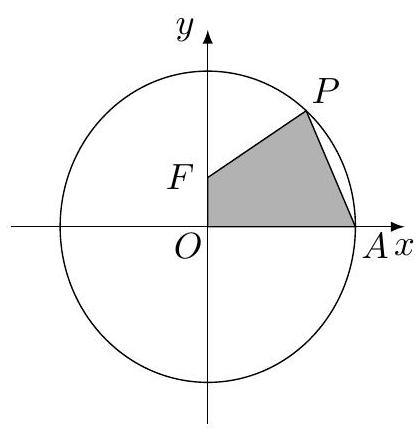
\includegraphics[max width=.3\textwidth, center]{2024_10_12_b4e0284229df56a127d4g-1}
  \item 若一个三位数中任意两个相邻数码的差均不超过 1 ,则称其为 "平稳数". 平稳数的个数是 \underline{\hspace{2cm}} .
  \item 正三棱雉 $P-A B C$ 中, $A B=1, A P=2$ ,过 $A B$ 的平面 $\alpha$ 将其体积平分,则棱 $P C$与平面 $\alpha$ 所成角的余弦值为 \underline{\hspace{2cm}} .
  \item 在平面直角坐标系 $x O y$ 中,点集 $K=\{(x, y) \mid x, y=-1,0,1\}$ 。在 $K$ 中随机取出三个点,则这三点中存在两点之间距离为 $\sqrt{5}$ 的概率为 \underline{\hspace{2cm}} .
  \item 在 $\triangle A B C$ 中, $M$ 是边 $B C$ 的中点, $N$ 是线段 $B M$ 的中点. 若 $A=\frac{\pi}{3}, \triangle A B C$ 的面积为 $\sqrt{3}$, 则 $\overrightarrow{A M} \cdot \overrightarrow{A N}$ 的最小值为 \underline{\hspace{2cm}} .\\
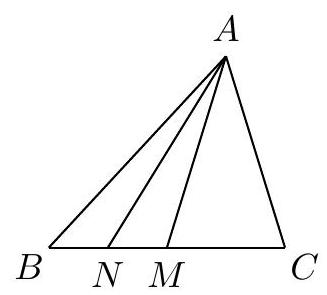
\includegraphics[max width=.3\textwidth, center]{2024_10_12_b4e0284229df56a127d4g-3}
  \item 设两个严格递增的正整数数列 $\left\{a_{n}\right\},\left\{b_{n}\right\}$ 满足: $a_{10}=b_{10}<2017$ ,对任意正整数 $n$ ,有 $a_{n+2}=a_{n+1}+a_{n}, b_{n+1}=2 b_{n}$ ,则 $a_{1}+b_{1}$ 的所有可能值为 \underline{\hspace{2cm}} .
\end{enumerate}

二、解答题:本大题共 3 小题,满分 56 分. 解答应写出文字说明、证明过程或演算步骤. 其中第 9 题满分 16 分, 第 10 、 11 题满分 20 分.
\begin{enumerate}
  \setcounter{enumi}{8}
  \item 设 $k, m$ 为实数, 不等式 $\left|x^{2}-k x-m\right| \leqslant 1$ 对所有 $x \in[a, b]$ 成立. 证明: $b-a \leqslant 2 \sqrt{2}$.
  \item 设 $x_{1}, x_{2}, x_{3}$ 是非负实数, 满足 $x_{1}+x_{2}+x_{3}=1$, 求 $\left(x_{1}+3 x_{2}+5 x_{3}\right)\left(x_{1}+\frac{x_{2}}{3}+\frac{x_{3}}{5}\right)$的最小值和最大值.
  \item 设复数 $z_{1}, z_{2}$ 满足 $\operatorname{Re}\left(z_{1}\right)>0, \operatorname{Re}\left(z_{2}\right)>0$, 且 $\operatorname{Re}\left(z_{1}^{2}\right)=\operatorname{Re}\left(z_{2}^{2}\right)=2$, 其中 $\operatorname{Re}(z)$ 表示复数 $z$ 的实部.
  (1) 求 $\operatorname{Re}\left(z_{1} z_{2}\right)$ 的最小值;\\
  (2) 求 $\left|z_{1}+2\right|+\left|\overline{z_{2}}+2\right|-\left|\overline{z_{1}}-z_{2}\right|$ 的最小值.
  
\end{enumerate}

\subsection*{二试}
一、如图, 在 $\triangle A B C$ 中, $A B=A C, I$ 为 $\triangle A B C$ 的内心. 以 $A$ 为圆心, $A B$ 为半径作圆 $\Gamma_{1}$, 以 $I$ 为圆心, $I B$ 为半径作圆 $\Gamma_{2}$, 过点 $B, I$ 的圆 $\Gamma_{3}$ 与 $\Gamma_{1}, \Gamma_{2}$ 分别交于点 $P, Q$ (不同于点 $B$ ). 设 $I P$ 与 $B Q$ 交于点 $R$. 证明: $B R \perp C R$.\\
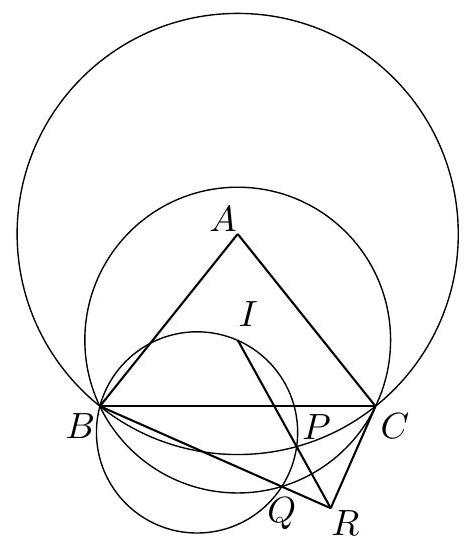
\includegraphics[max width=.3\textwidth, center]{2024_10_12_b4e0284229df56a127d4g-5}

二、设数列 $\left\{a_{n}\right\}$ 定义为 $a_{1}=1$ ,

求满足 $a_{r}<r \leqslant 3^{2017}$ 的正整数 $r$ 的个数.

三、将 $33 \times 33$ 方格纸中每个小方格染三种颜色之一,使得每种颜色的小方格的个数相等.若相邻两个小方格的颜色不同,则称它们的公共边为 "分隔边". 试求分隔边条数的最小值.

四、设 $m, n$ 均是大于 1 的整数, $m \geqslant n . a_{1}, a_{2}, \cdots, a_{n}$ 是 $n$ 个不超过 $m$ 的互不相同的正整数, 且 $a_{1}, a_{2}, \cdots, a_{n}$ 互素。证明:对任意实数 $x$ ,均存在一个 $i(1 \leqslant i \leqslant n)$ ,使得 $\left\|a_{i} x\right\| \geqslant \frac{2}{m(m+1)}\|x\|$, 这里 $\|y\|$ 表示实数 $y$ 到与它最近的整数的距离.


\end{document}